\documentclass{beamer}
\usetheme{SLAC}

\usepackage[utf8]{inputenc}
\usepackage[T1]{fontenc}
\usepackage[babel]{csquotes}
\usepackage{lmodern}
\usepackage{graphicx}
\usepackage{xcolor}
\usepackage{amsmath, amsfonts, amssymb, amsthm, bbm}
\usepackage{listings}
%\usepackage{array}
%\usepackage{ifthen}
%\usepackage{pgf, tikz, pgfplots}
%\pgfplotsset{compat=1.12}
%\usepgfplotslibrary{units, fillbetween}
%\usetikzlibrary{spy, arrows,shapes,backgrounds, calc, fadings, decorations, automata, positioning, mindmap, shadows, decorations.pathreplacing, decorations.pathmorphing}
%\usepackage{appendixnumberbeamer}  % \appendix
%\usepackage{pgfpages} %needed for notes on second screen
\usepackage{pdfpages}
%\usepackage{multimedia}  % \movie
\usepackage{hyperref}


%Information to be included in the title page:
\title{SLAC}
\subtitle{Latex Beamer Template with a really long subtitle such that it spans over multiple lines}
\author{Stephan Kuschel}
\institute{SLAC National Accelerator Laboratory}
\date{\today}



\begin{document}


\frame{\titlepage}


\begin{frame}[fragile]
\frametitle{What is this template?}
\begin{itemize}
\item This is an \underline{inofficial} \LaTeX-beamer template for SLAC.
\item The official PowerPoint template can be found here: \\
\url{https://portal.slac.stanford.edu/sites/lcls_public/Documents/ppt-template-white-July26.pptx}
\end{itemize}
In case this has been downloaded from github, here is some version information: \\
Date: \verb|$Format:%ci$| \\
git sha: \verb|$Format:%H$| \\[1em]
The current version can be found at:
\url{https://github.com/skuschel/slac-beamer-template}
\end{frame}


\begin{frame}{Lists and Items}
  \begin{itemize}
    \item item of first level
    \begin{itemize}
      \item item of second level
      \begin{itemize}
        \item item of third level
      \end{itemize}
    \end{itemize}
  \end{itemize}
  \begin{enumerate}
    \item one
    \item two
    \item three
  \end{enumerate}
\end{frame}

\begin{frame}{blocks}
\begin{block}{block}
  blocktext
\end{block}

\begin{alertblock}{alertblock}
  blocktext
\end{alertblock}

\begin{exampleblock}{exampleblock}
  blocktext
\end{exampleblock}

Finally, use an exampleblock with an empty title to recreate the block from the official template:
\begin{exampleblock}{}
  blocktext
\end{exampleblock}
\end{frame}


\begin{frame}{Image ressources}
Images can be found here:
\begin{itemize}
  \item SLAC's official Flickr channel: \\
  \url{www.flickr.com/photos/slaclab/albums}
  \item Stanfords phot archive: \\
  \url{www.sallie.stanford.edu}
\end{itemize}
\end{frame}


\setlength{\unitlength}{\paperwidth}%
\usebackgroundtemplate{%
\begin{picture}(1,0.75)%
\put(0,0){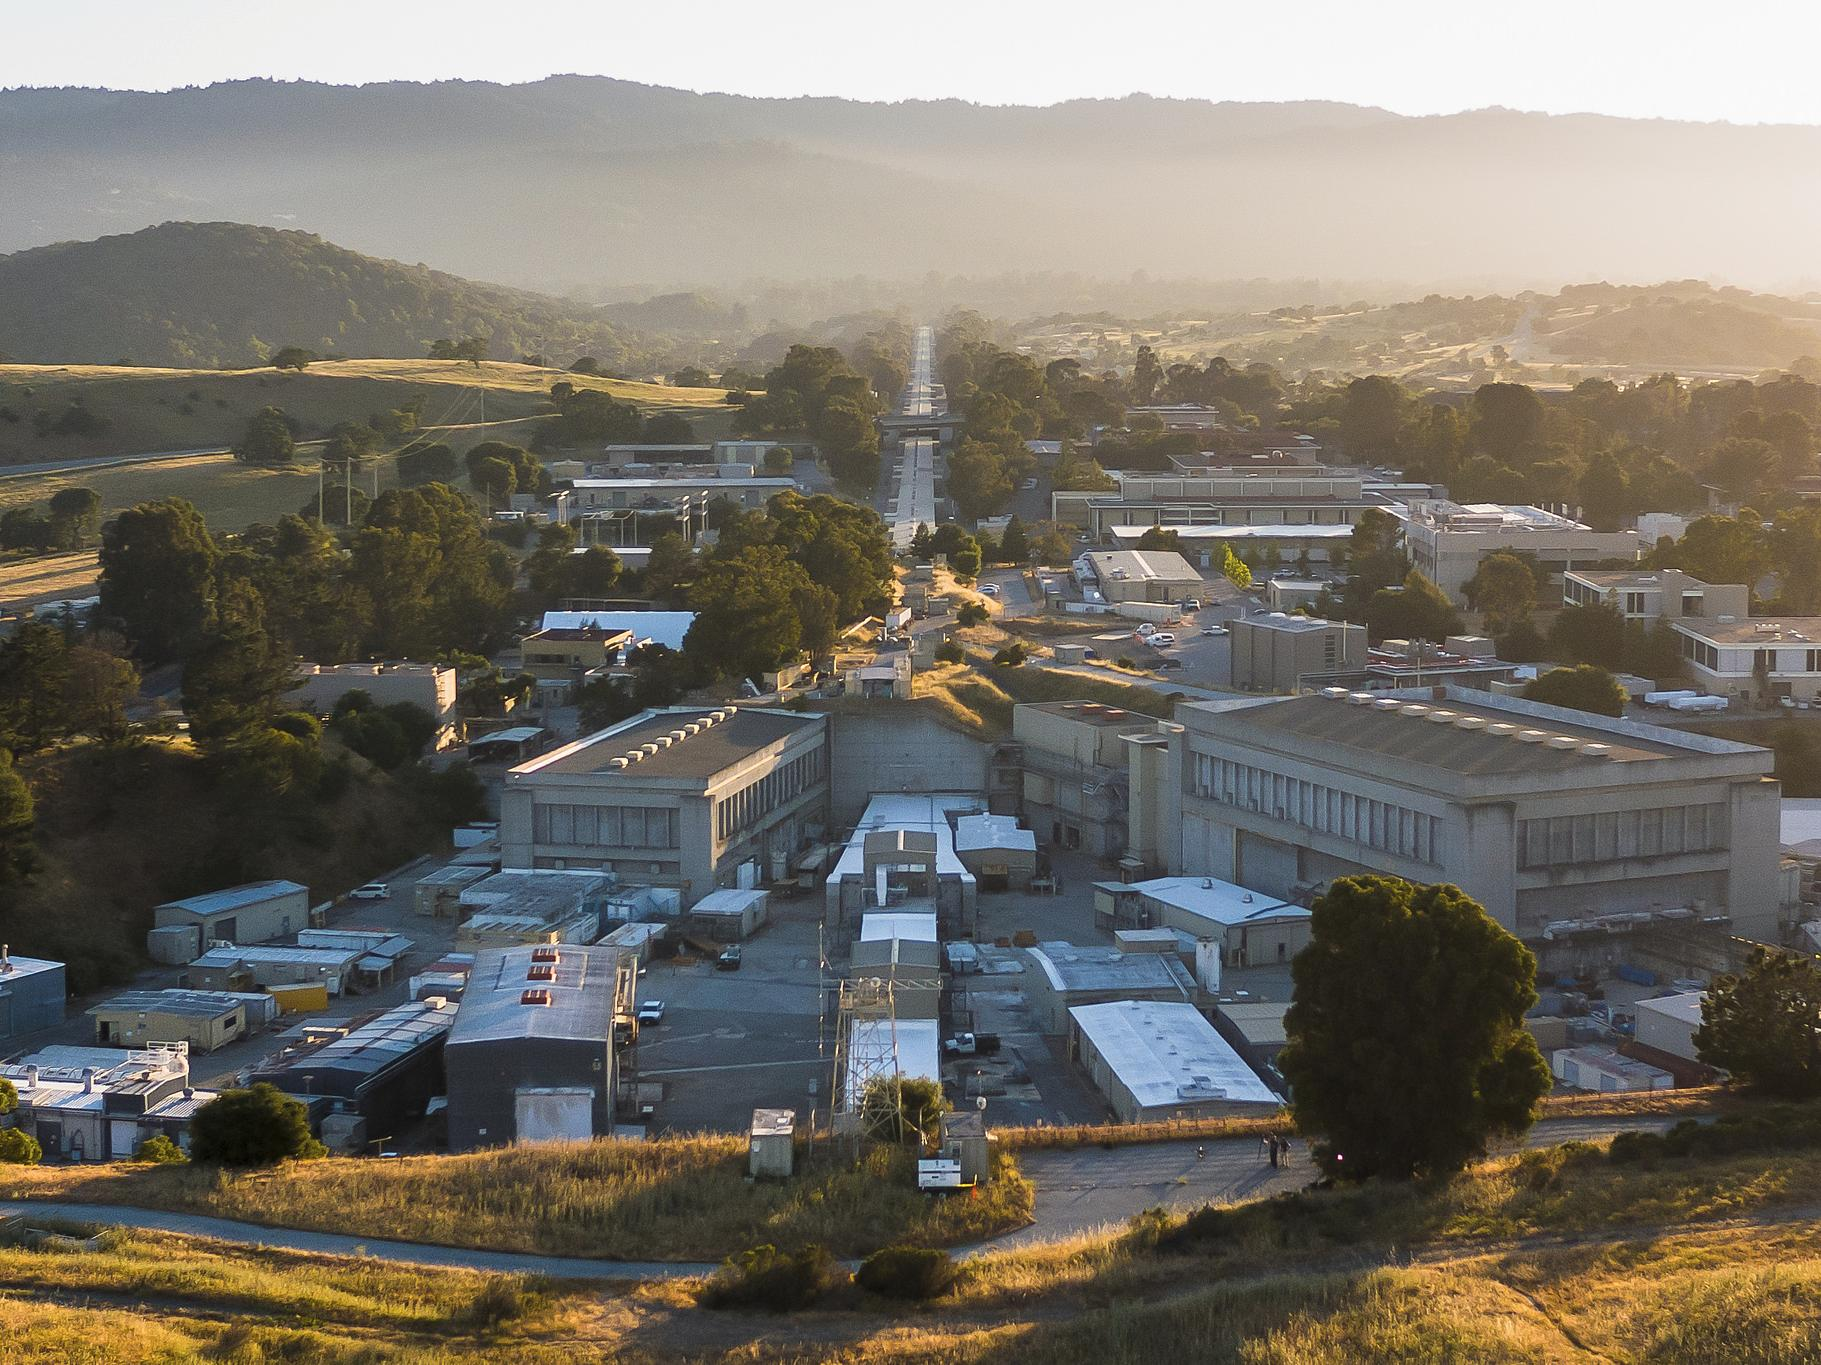
\includegraphics[width=\paperwidth]{slac-divider.jpg}}
\put(0,0){
\includegraphics[width=\paperwidth]{slac-lines-white.png}}
\put(0.83,0.04){
\includegraphics[width=1.4cm]{slac-logo-white.png}}
\end{picture}
}
\begin{frame}
\textcolor{white}{
\begin{center}
  \LARGE \bfseries Divider page
\end{center}}
\end{frame}
\usebackgroundtemplate{}

\end{document}
